\section{Early days of the Internet and its remaining flaws}\label{early}

The need to build a global communications network in an age when almost nobody had access to that technology and the unpredictability of the number of future users, lead to some protocols not being suitable for the explosive growth and proliferation of users that followed. \ac{IPv4} limits the number of public addresses in such a way that today they are scarce \cite{ipv4}. {\color{blue} Today we live in the \emph{Internet of Things} era.
  Users and companies may have multiple devices that require Internet connectivity, such as personal computers, smart phones, tablets, traffic sensors, public vigillance systems, health monitoring tools and so on. All those devices combined cannot be publicly addressed by \ac{IPv4}.}
%RP vigillance -> surveilance?
%RP usa acrónimo IoT para Internet of Things

To this end, one way to overcome the \ac{IPv4} address scarcity problem was the development of a mechanism that groups multiple address into a single one, the machine that is assigned that address is then responsible for redirecting messages to members of its group using their private addresses, each connection in the private network is identified publicly by the same \ac{IP} address with a different port.
%RP o porto não identifica uma máquina (membro da rede privada) mas uma ligação.
This technique is known as \ac{NAT}.

\begin{figure}[H]
	\centering
	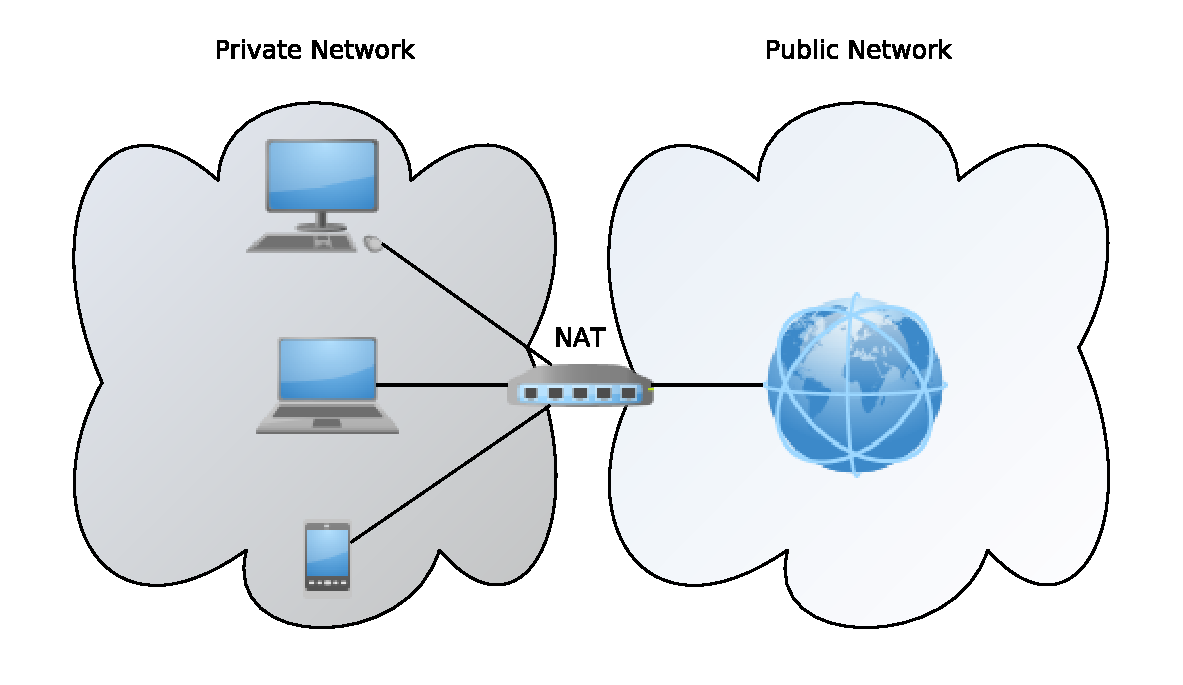
\includegraphics[width=0.7\textwidth]{figures/nat.pdf}
	\caption{Network Address Translation}
\end{figure}
%RP na figura devias indicar que uns tem ips publicos e outros privados. Alternativamente, colocavas metade da nat box dentro da núvem para indicar que esta pertence à Internet e os pc não. 

Initially \ac{NAT} offered an alternative to address exhaustion and a minimal sensation of security.
However, due to their current wide usage, \ac{NAT}s weaknesses are being exposing at the application layer, {\color{blue}namely impacting applications that require direct communications between two private networks.}

There are four types of \ac{NAT} implementations\cite{rfc3489}: \emph{Full Cone NAT}, \emph{Restricted Cone NAT}, \emph{Port Restricted Cone NAT}, \emph{Symmetric NAT}.

\emph{Full Cone} \ac{NAT} maps each public \ac{IP} address and port to a private \ac{IP} address and port.
Any external host can communicate with private hosts through their mapped public address and port. This represents the least restrictive type of \ac{NAT} and, as we will see later, the unique type of \ac{NAT} that enables real time communications from point to point.

\emph{Restricted Cone} \ac{NAT} requires that a private client must first send a message to an external host before it can receive messages from the same host. With this type of \ac{NAT}, the private client can be contacted from any port of the same external host.

\emph{Port Restricted Cone} \ac{NAT} works in the same way as Restricted Cone \ac{NAT}, but it only allows communications from the same external host's IP address and port, ignoring all messages from other applications within the same external host.

\emph{Symmetric} NAT maps different ports for each connection. As we will see later, this type of \ac{NAT} represents a problem on real time communications.

\emph{Non-Symmetric} \ac{NAT}s became the common configurations on the Internet. As a direct result, problems started to appear: the amount of ports that \ac{IP} makes available is also small compared to our current needs; worse than that, \ac{NAT} also difficults end-to-end communication, forcing most applications that follow this model to be implemented ineffectively.

{\color{blue}Unless the router that performs as \ac{NAT} has forwarding rules to every desired ports of each user}, applications behind a \ac{NAT} are prevented from receiving incoming connections from the public network, which forces them to behave as a client of a client-server model. 

%RP explicar que o nat funciona num cenário em que a máquina atrás do nat é apenas um consumidor de informação, trabalhando em modo cliente do modelo cliente-servidor. Em P2P isto falha.

Applications based on multimedia and peer-to-peer file sharing have been one of the most strained by the \ac{NAT} technique. It is also important to highlight that those kind of applications require real time communication in order to achieve the best performance.

\begin{figure}[H]
	\centering
	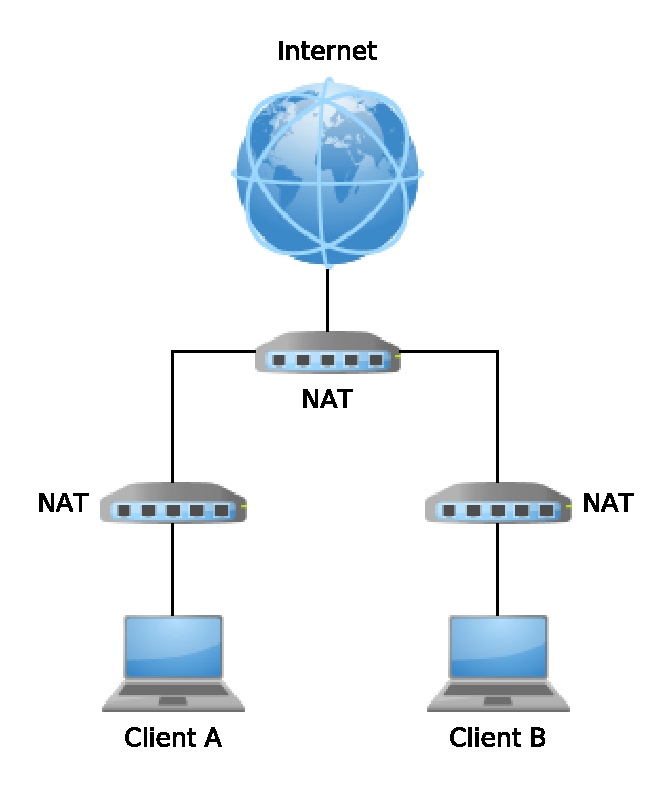
\includegraphics[width=0.45\textwidth]{figures/multinat.pdf}
	\caption{Multiple level NATs}
\end{figure}

%RP file sharing não precisa de real-time
\ac{STUN} and \ac{TURN} \cite{natvoip} servers are a possible solution to overcome \ac{NAT}. None of those can establish direct connections on multiple level \ac{NAT}s.
%HR XXX I was here
%RP explicar o que são multiple level pois não falaste disto antes? São ``nested''?

\ac{STUN} servers are quite simple. They receive requests from \ac{NAT}ed clients, with the source address of a request being the public address that \ac{NAT} mapped to the client. \ac{STUN} servers will then reply to the client, providing the mapped public address, so it knows its associated public \ac{IP} address and port. Symmetric \ac{NAT} changes \ac{IP} port for each different connection, for that reason, when the \ac{STUN} servers reply with the \ac{IP} address and port of their connection, it will be useless for clients to use them on other application connections. That is why Symmetric \ac{NAT} represents a problem for peer-to-peer communications.   
%RP os problemas que relatas têm a ver com P2P ou real-time?

On the other hand, \ac{TURN} uses public servers to relay traffic between private endpoints.
It may use a \ac{P2P} network relay to find the best peer, but after that, the behavior is much like client-server. Direct communication is only achieved by \ac{STUN} when \ac{NAT} is a type \emph{full cone}. \ac{ICE} is a technique that uses \ac{STUN} when direct communications are possible and \ac{TURN} while a direct communication isn't possible.
%RP ainda não explicaste o que é o ICE
%RP explicar que para usar TURN as aplicações têm de estar cientes disso.

Most of client-server applications aren't affected by \ac{NAT} when the servers are public, but they're inadequate for real time communication between two private endpoints. Clearly \ac{TURN} requires a more expensive relaying infrastructure and, in most cases, more network usage, leading to a worse quality of service. The requirements of real-time video communication makes this kind of model unsuitable.
%RP quando falas em infraestrutura mais dispendiosa para o video, está a falar da internet ou ainda estamos a falar de usar ICE?


When connection is established, either in a direct or indirect way (via \ac{TURN} servers), \ac{WebRTC} came to simplify how audio and video are transmitted through web browsers.
